\chapter{Introducción}


\section{Fundamentos teóricos de la luz}

\subsection{Radiación electromagnética}

La luz es radiación electromagnética que se propaga como onda a través del espacio transportando energía radiante en el proceso. Está constituida por partículas elementales sin masa denominadas fotones.
Las propiedades de la luz están condensadas en el espectro electromagnético (Figura~\ref{espectroelectromagnetico}) con base en el número de oscilaciones de la onda por unidad de tiempo (frecuencia) y la distancia lineal entre dos puntos equivalentes de ondas sucesivas (longitud de onda).\\

\begin{figure}
  \centering
    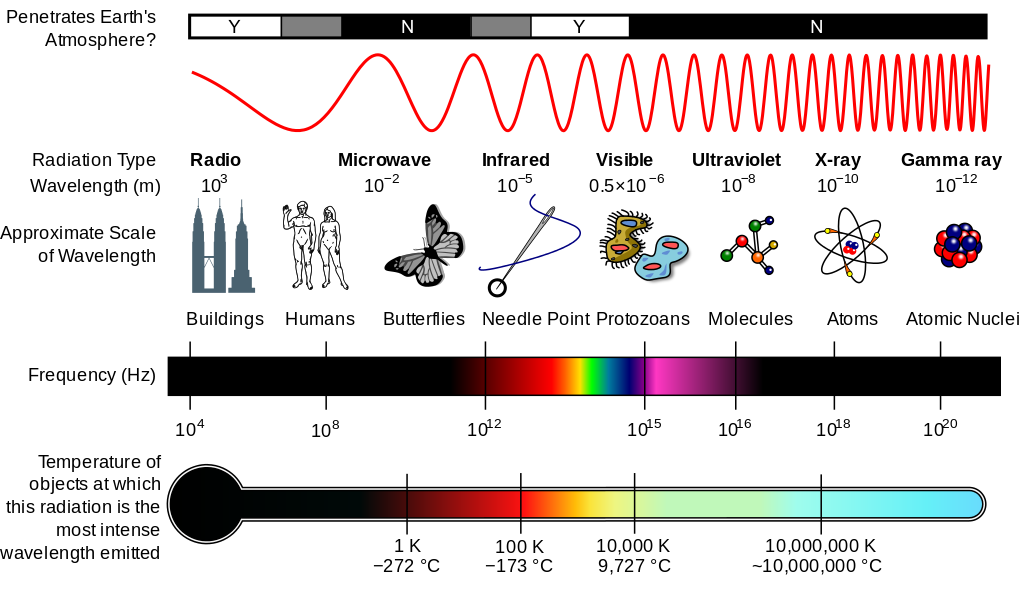
\includegraphics[width=1\textwidth]{espectroelectromagnetico}
  \caption{Espectro electromagnético \citep{NASA2007}}
  \label{espectroelectromagnetico}
\end{figure}

Una de tales propiedades, importante para este trabajo en la región visible del espectro electromagnético ($\sim$ 450-750 nm), es la temperatura de color que está definida a partir de la Ley de desplazamiento de Wien. Esta ley explica la relación inversa entre la longitud de onda en la que se produce el pico de emisión de un cuerpo negro y su temperatura:

\begin{equation}
\lambda_{max}=\dfrac{b}{T}
\end{equation}


Propiedades de propagación

\subsection{Unidades de medición de la luz}

Métodos experimentales

Métodos teóricos

Para la estimación regional de la CL se puede optar por alguno de los métodos arriba descritos o incluso la combinación de ambos.\\

Las magnitudes son unidades astronómicas de medición permiten establecer una escala de brillo aparente de objetos celestes. Algunos ejemplos (de menos a más brillantes)son:

\begin{itemize}

    \item 0.03. Vega, la estrella de referencia
    \item 6. Estrellas perceptibles a simple vista
    \item -12.6. Luna llena
    \item -26.73 Sol
    
 \end{itemize}
 
 Para la medición del brillo del cielo nocturno se utilizan diferentes unidades según el enfoque del estudio. En el caso de estudios generales (sin dependencia espectral) se retoman las magnitudes astronómicas por unidad de área.\\
 
En este sentido las magnitudes/arcosegundo se definen como el brillo medido en magnitudes extendido sobre un arcosegundo cuadrado del cielo (área).\\

Hay 360 grados en un círculo, hay 60 arcominutos en un grado, hay 21,600 arcominutos en un círculo. Hay 60 arcosegundos en un arcominuto, hay 1,296,000 arcosegundos en un círculo.\\

Estas unidades de medición son logarítmicas (lo que implica que cambios pequeños en la medición reflejan cambios grandes en el brillo del cielo).\\

El uso de esta unidad de medición requiere de ciertas consideraciones para la interpretación correcta de los resultados. Como se mencionó con anterioridad, las nubes, el aerosol atmosférico,la niebla y la neblina pueden alterar las mediciones tanto de campo como las remotas.



En \textit{Caracterización de la contaminación lumínica en zonas protegidas y urbanas} (2015), tesis doctoral de Salvador Ribas de la Universidad de Barcelona, se menciona dos tipos de medición del brillo del cielo nocturno:

\begin{itemize}

    \item Extensivas (a lo largo de un territorio)
    \item Continuas (emplazamiento permanente a lo largo de una red)     
    
\end{itemize}

En ambos casos, la finalidad óptima es la elaboración de un mapa de niveles de contaminación lumínica que incluya la dimensión temporal para evaluar los cambios en el brillo del cielo nocturno.\\

La red de Contaminación Lumínica Catalana es un ejemplo de medición continua de la CL.


\section{Brillo del cielo nocturno}

\subsection{Componentes del brillo del cielo nocturno}

De acuerdo con Leinert at.al (1998), el brillo total $(I_{tot})$ del cielo nocturno puede calcularse a partir de la siguiente ecuación:

\begin{equation}\label{eq:ej}
I_{tot}=(I_A + I_{ZL} + I_{ISL} + I_{DGL} + I_{EBL})\ exp \ (-\tau) + I_{SCA}
\end{equation}

Donde $\tau$ es el coeficiente de extinción que depende de la longitud de onda, el ángulo cenital, la altura sobre el nivel del mar y la composición atmosférica del lugar de la observación.


\subsection{Variación natural del brillo del cielo nocturno por influencia de objetos astronómicos}

\subsection{Variación natural del brillo del cielo nocturno por influencia de las condiciones atmosféricas}

\subsubsection{Propiedades ópticas de las nubes}

\subsubsection{Propiedades ópticas del aerosol atmosférico}


\section{Importancia del ciclo día-noche en la evolución de la vida}

La duración del ciclo día-noche en la Tierra ha cambiado significativamente a lo largo de la historia geológica debido a la variación de la rotación del planeta. La velocidad de rotación original de los planetas  es consecuencia de la conservación del momento angular que poseía la nebulosa interestelar que, al colapsar, dio origen al Sistema Solar hace aproximadamente 4600 Ma \citep{Greaves2005}. Sin embargo, si la hipótesis del Impacto de Theia es correcta, es factible que la rotación primordial de la Tierra haya sido reconfigurada hace alrededor de 4500 Ma, cuando un cuerpo astronómico del tamaño de Marte, nombrado Theia, colisionó tangencialmente con nuestro planeta dando origen, además, a la Luna \citep{Stevenson1987}.\\

La masa lunar es lo suficientemente grande y cercana con respecto a la Tierra para ejercer atracción gravitatoria significativa sobre los océanos, generando así abultamientos de masas de agua (mareas) en ambos extremos del planeta alineados con el eje Tierra-Luna. Sin embargo, la rotación terrestre ocasiona el arrastre de las mareas hacia delante del mencionado eje, lo que implica que una fracción de la atracción gravitatoria Tierra-Luna está desfasada y da origen al torque lunar $\uptau_0$ que reduce la velocidad de rotación de la Tierra \citep{Conway1982}.\\ 

Como se muestra en la Figura~\ref{duraciondia}, la duración que tuvo el día terrestre posterior a la gran colisión de Theia debió de ser de tan sólo 7 horas aproximadamente gracias a la gran velocidad de rotación y el cambio en la inclinación del eje de rotación que el planeta llegó a experimentar luego del evento \citep{Stevenson&Bartlett2016}, \citep{Stevenson1987}; con el paso de los millones de años, tal velocidad fue disminuyendo como consecuencia del torque lunar \citep{Conway1982}.\\ 

El periodo estable de duración del día terrestre de 21 horas que se mantuvo durante gran parte del Precámbrico (Figura~\ref{duraciondia}) se explica con la llamada Hipótesis de Estabilización Resonante \citep{Zahnle&Walker1987}, la cual sostiene que, durante algún tiempo, el anteriormente mencionado torque lunar pudo haber sido cancelado por un torque de signo contrario originado por la resonancia entre las mareas atmosféricas semi-diurnas térmicamente accionadas y las oscilaciones libres de la atmósfera.\\

\begin{figure}
  \centering
    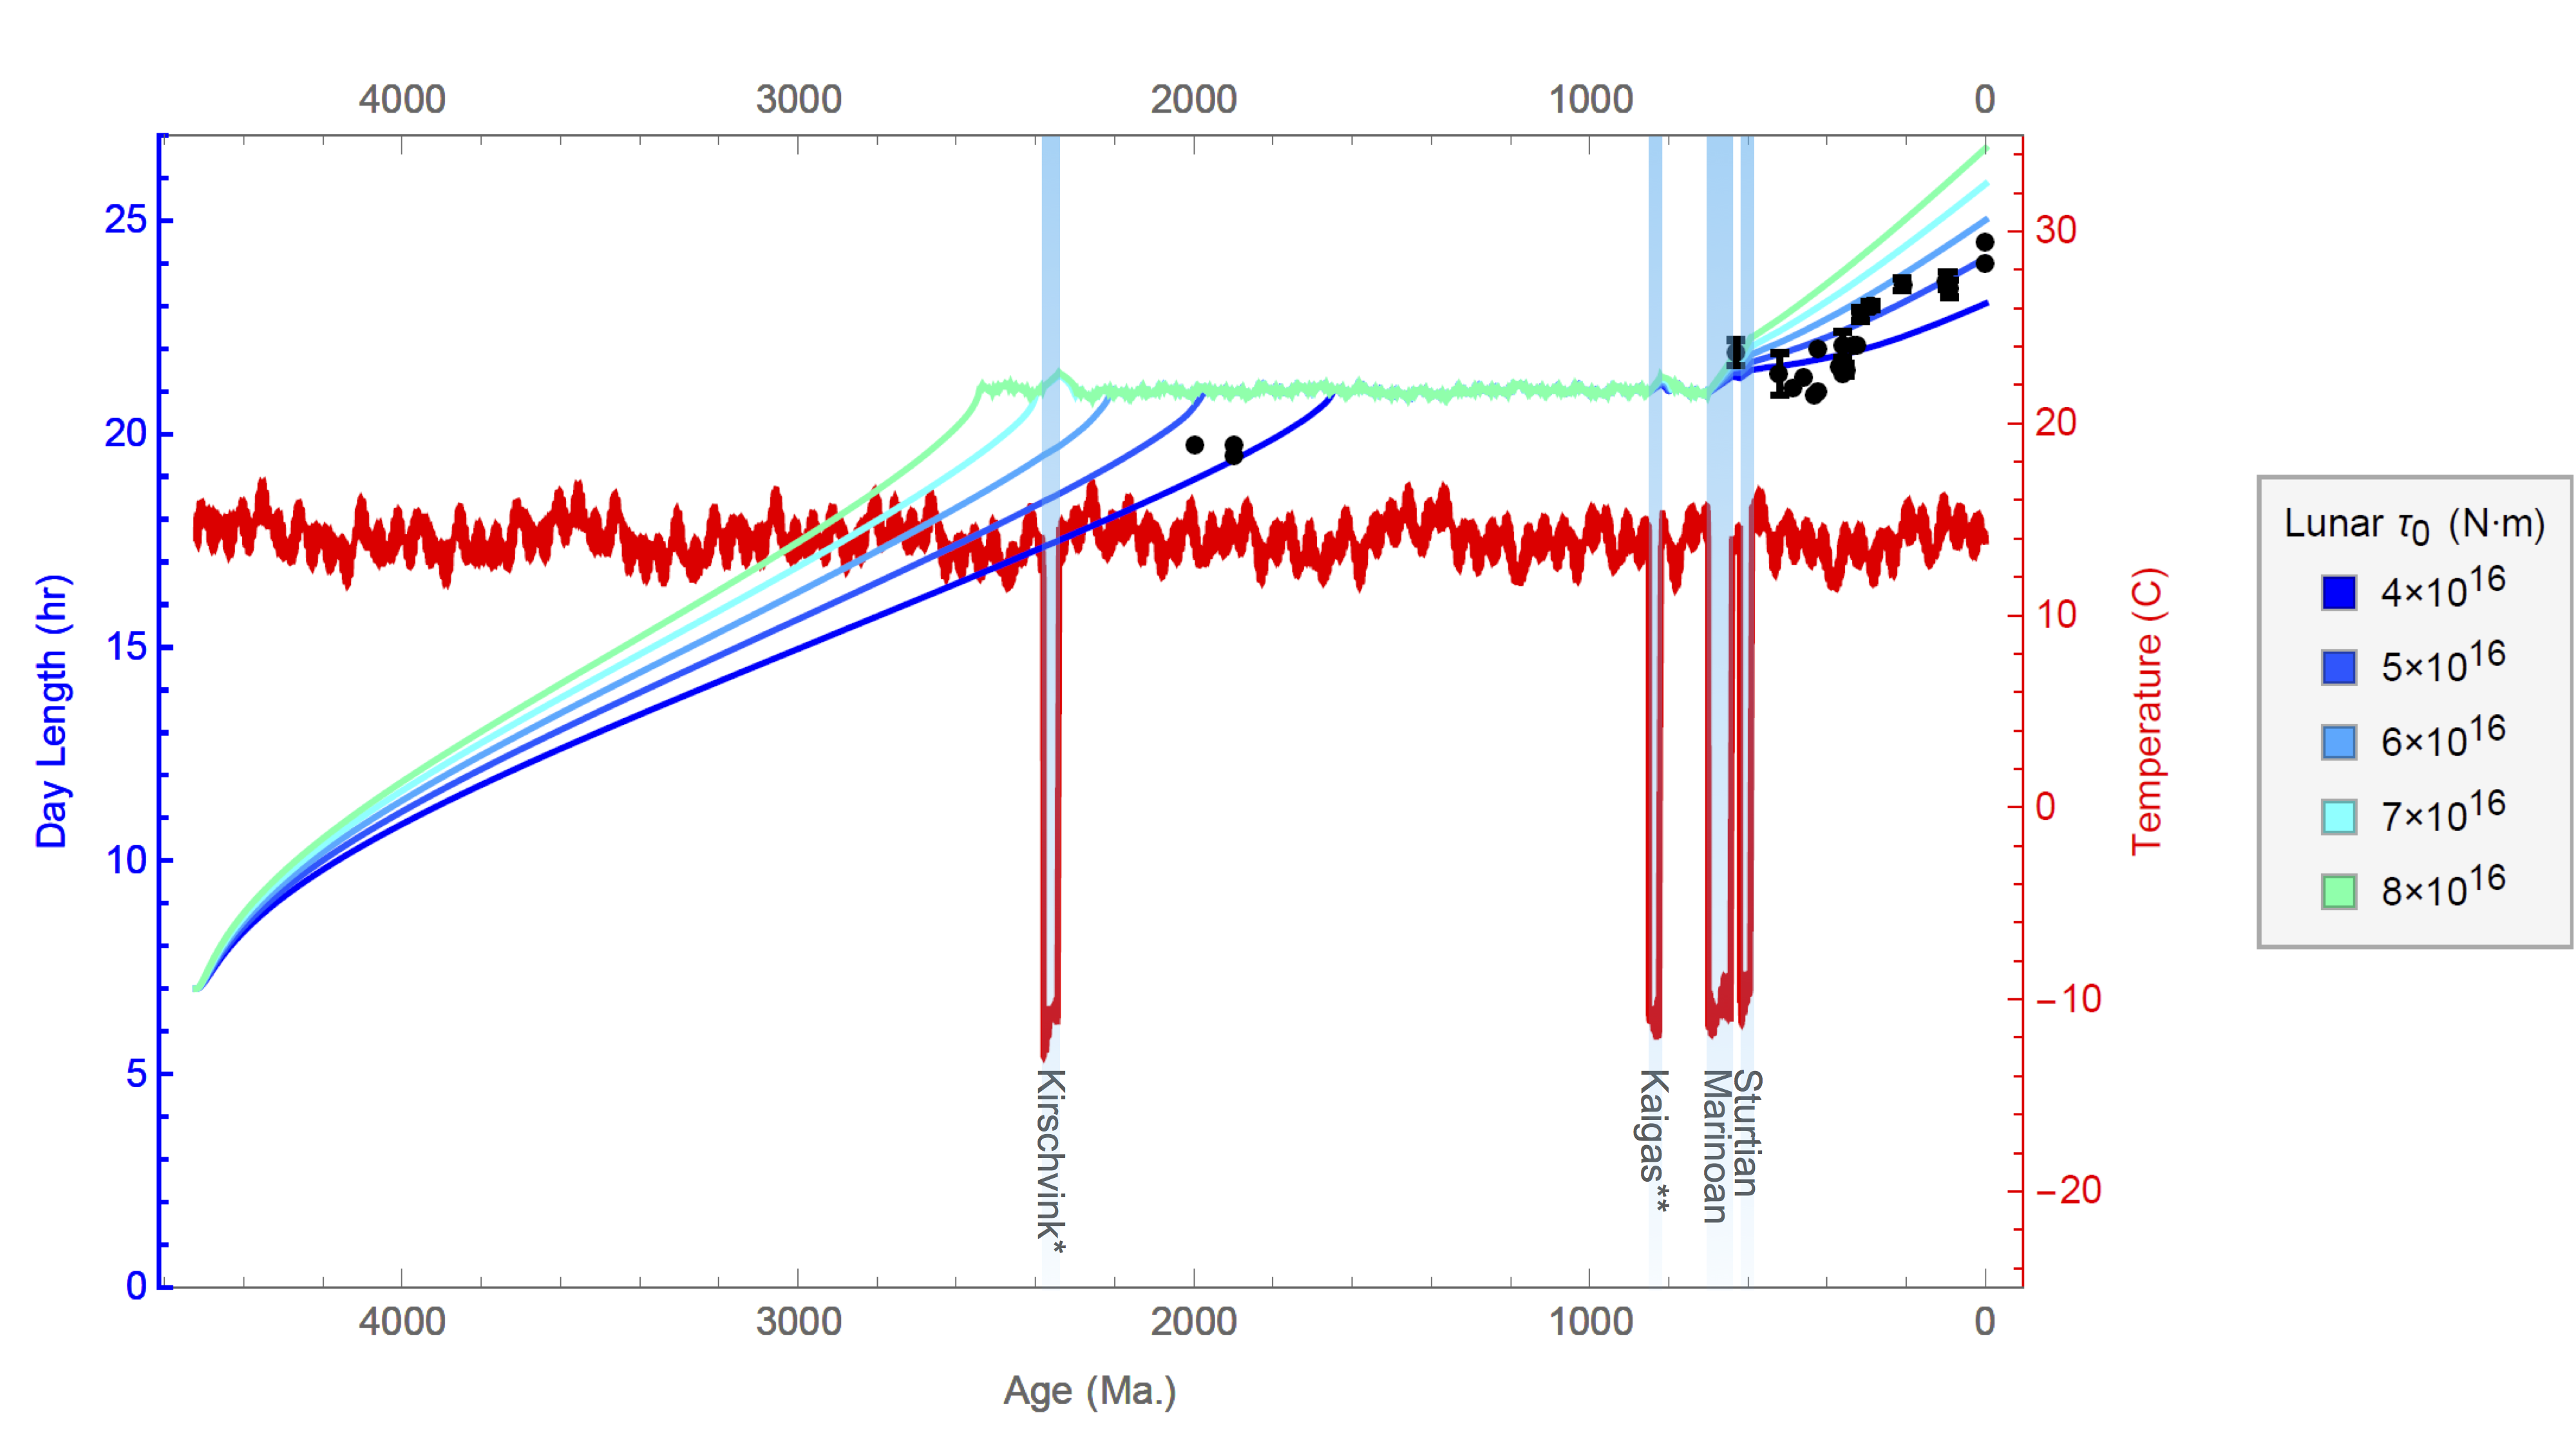
\includegraphics[width=1\textwidth]{duraciondeldiahistorico}
  \caption{Simulación de la historia geológica de la duración del día terrestre \citep{Stevenson&Bartlett2016}}
  \label{duraciondia}
\end{figure}

La velocidad de rotación actual de la Tierra debió comenzarse a perfilar hace aproximadamente 600 Ma cuando las grandes glaciaciones de ese entonces pudieron haber desestabilizado térmicamente el torque atmosférico, por lo que actualmente, el torque lunar sigue siendo lo suficientemente considerable como para continuar disminuyendo la velocidad del planeta \citep{Stevenson&Bartlett2016}. Para el final del Criogénico, el ciclo día-noche tomó, finalmente, su configuración actual al mismo tiempo que los niveles de oxígeno y ozono estratosférico fueron óptimos para el surgimiento y desarrollo de vida más compleja (multicelular) en un evento conocido como \textit{la Radiación del Cámbrico}, durante el que se originaron y diversificaron la mayoría de los filos animales incluyendo el de los cordados, al que pertenecemos los humanos.\\

$https://en.wikipedia.org/wiki/Cambrian_explosion$	
Poner la gráfica de Holker. Oscuridad, ventaja evolutiva. Más horas de noche, mayor nocturnidad con el paso del tiempo.\\

\section{Contaminación lumínica}

\subsection{El enfoque socioecosistémico}

Socioecosistema\\

1. Socioecosistema IES\\

2. De ecosistema a socioecosistema diseñado
como territorio del capital agroindustria\\

3. Sistemas socio-ecológicos: elementos teóricos y conceptuales para la discusión en torno a vulnerabilidad hídrica.\\

Uso y abuso de la energía\\

\subsection{Contexto histórico del estudio de la CL}

\subsection{Tipos de CL}

\subsection{Consecuencias de la CL}

En qué región del espectro se ven afectadas diferentes clases de animales de acuerdo con su visión (luminancia).\\

\subsection{Marco regulatorio: normas y leyes en México y el mundo}

Ley 31/1998 Protección de la Calidad Astronómica de los Observatorios del Instituto de Astrofísica de Canarias.\\

Ley 6/2001 Ordenación ambiental del alumbrado para la protección del medio nocturno.\\

Zonificación con 4 categorías y una especial.\\

\begin{itemize}

    \item E1. Espacios que por sus características naturales o su valor astronómico especial, sólo se puede admitir un brillo mínimo.
    
    \item E2. Áreas incluidas en ámbitos territoriales que sólo admiten un brillo reducido.
    
    \item E3. Áreas incluidas en ámbitos territoriales que admiten un brillo medio
    
    \item E4. Áreas incluidad en ámbitos territoriales que admiten un brillo alto.
    
    \item Puntoa de referencia. Puntos cercanos a las áreas de valor astronómico o natural especial incluidos en E1, para los que hay que establecer una regulación específica en función de la distancia a la que se encuentren del área en cuestión.
    
    
\end{itemize}

Según el Departamento de Estudios Luminotécnicos de la ETSEIB (UPC) en \textit{Evaluación del Impacto Ambiental Lumínico en Zonas Protegidas del Área Metropolitana de Barcelona}, los aspectos importantes para controlar la Contaminación Lumínica son:

\begin{itemize}
    \item Niveles más estrictos a los permisos de las luminarias (Comité Internationale d'Eclairage)
    
    \item Límites de luminosidad en el espacio-tiempo (periodo de protección especial a partir de las 23 hrs.)
    
     \item Cambiar el uso de luz blanca (especialmente nociva) a una temperatura de color neutra (4200 K), promoviendo las cálidas (inferiores a 3000 K)
     
\end{itemize}

\section{Alumbrado público}

\subsection{Fuentes de luz}

\subsection{Tipos de luminarias}

\subsection{Función de emisividad urbana}


\section{Estudio de caso: Ciudad de México}

\subsection{Descripción del área de estudio}

Incluir REPSA

\subsection{Inventario de alumbrado público}

\subsection{Consumo de energía eléctrica}

Datos de consumo de energía eléctrica por entidad federativa por el Sistema de Información Energética de la Secretaría de Energía.\\

\subsection{Climatología de nubes y aerosol atmosférico}

\section{Hipótesis}

\section{Objetivos}

\subsection{Generales}

\begin{itemize}

    \item Reproducir el modelo \textit{SkyGlow} para el caso de la Ciudad de México
    
    \item Estimar los niveles de contaminación lumínica en la Ciudad de México 
    
    \item Generar un antecedente para la campaña de validación del modelo \textit{SkyGlow} en la Ciudad de México
    
\end{itemize}

\subsection{Particulares}

\begin{itemize}

    \item Caracterizar el alumbrado público de la Ciudad de México 
    
    \item Elaborar un mapa teórico de contaminación lumínica de la Ciudad de México bajo condiciones de cielo despejado
    
    \item Construir mediante simulaciones diferentes escenarios del brillo del cielo nocturno tomando en cuenta diferentes posiciones del observador y condiciones atmosféricas
    
    \item Inferir la influencia del aerosol atmosférico  y la nubosidad en el brillo del cielo nocturno a partir del objetivo anterior
    
    
\end{itemize}